\documentclass[12pt,A4, onecolumn]{exam}
\usepackage{amsmath}
\usepackage{amssymb}
\usepackage{epstopdf}
\usepackage[lmargin=71pt, tmargin=1.2in]{geometry}  %For centering solution box
\lhead{TEK4090 -- Introduction to Modern Control\\}
\rhead{Assignment 2\\}
% \chead{\hline} % Un-comment to draw line below header
\thispagestyle{empty}   %For removing header/footer from page 1

\usepackage{gensymb}
\usepackage{graphicx}
\usepackage{hyperref}
\graphicspath{{../../figs/}}
\epstopdfsetup{outdir=../../figs/}

\def\showsoln{1}

\begin{document}

\begingroup  
    \centering
    \LARGE TEK4090 -- Introduction to Modern Control\\
    \LARGE Assignment 2 v4.0\\[0.5em]
    \large Due: October 23 2024, 13:15\\
\endgroup
\rule{\textwidth}{0.4pt}
%\pointsdroppedatright   %Self-explanatory
\printanswers


\renewcommand{\solutiontitle}{\noindent\textbf{Ans:}\enspace}   %Replace "Ans:" with starting keyword in solution box

\begin{questions}

\begin{question}[10]
  Consider the continuous-time system,
  \begin{align}
    \ddot x &= u\\
    J(t_0) & = \dfrac{1}{2}x^2(0) + r\int_0^2 u^2dt.
  \end{align}
Hint: read \S6.3 in Lewis, Syrmos, \& Vraibie for some relevant example problems
  \begin{parts}
    \part Write the Hamilton-Jacobi-Bellman (HJB equation), eliminating $u(t)$ 

    \begin{solution}
      We begin by writing the hamiltonion equation:

      \[
          H(x, u, \lambda, t) = ru^2 + \lambda^T f(x,u,t)
      \]

      Where $ \lambda \in \mathbb{R}^2$. We define f as a vector in $ \mathbb{R}^2 $ as well where 
      
      \[
          f =\begin{bmatrix}
             x_2\\
             u 
          \end{bmatrix} 
      \]

      if we take $ \dot{x} = x_2 $ and $ \dot{x_2}=u $. We not get that the Hamiltonion is
      \[
          H=ru^2 + \lambda _1x_2 + \lambda _2u
      \]
      
      Our goal is to find the Hamilton Jacobi equation, 

      \[
          -J_t^* = min_u \left( ru^2+ \lambda _1x_2 + \lambda _2u\right) 
      \]
      which we find by optimizing H for u and substituting the optimal u in H. First note that $ \frac{ \partial^2 H }{ \partial u^2 } = 2r \ge 0 $, which is a condition for global convexity, assuming $ r \ge 0 $ . This means that the optimal $ u^* $ we find is the global minimum of the Hamiltonion.

      \begin{align*}
        \frac{ \partial H }{ \partial u } &= 0 \\
        &= 2ru + \lambda _2 \\
        u^* &= - \frac{ \lambda_2 }{ 2r }
      \end{align*}

      We now substitute optimal control into h
      \begin{align*}
        H^* &= r \left( - \frac{ \lambda _2 }{ 2r } \right)^2 + \lambda _1 x_2 - \frac{ \lambda _2^2 }{ 2r } \\
        &= \frac{ \lambda _2 }{ 4r } + \lambda _1 x_2 - \frac{ \lambda _2^2 }{ 2r } \\
        &= \frac{ - \lambda _2^2 }{ 4r } + \lambda _1 x_2
      \end{align*}
      
      Substituting this into $ J^* $ we get that 
      
      \[
          -J_t^* = min_u \left( ru^2+ \lambda _1 x_2 + \lambda _2 u \right) = \frac{ - \lambda _2^2 }{ 4r } + \lambda _1 x_2 
      \]
      
      
    \end{solution}

    \part Assume that the optimal cost-to-go function $J^*(t)$ is given by,
      \begin{align}
        J^*(t) = \dfrac{1}{2} s_1(t)x^2(t) + s_2 (t)x(t)\dot x(t) + \dfrac{1}{2} s_3 (t)\dot x^2 (t).
      \end{align}
      Use the HJB equation to derive coupled differential equations for these $s_i(t)$'s, and find boundary conditions for these equations.

      \begin{solution}
        We find that 

        \begin{itemize}
          \item $ \lambda _1 = \frac{ \partial J^* }{ \partial x } = s_1x + s_2 \dot{x} $
          \item  $ \lambda _2 = \frac{ \partial J^* }{ \partial \dot{x} } = s_2x + s_3 \dot{x} $
          \item $\frac{ \partial J^* }{ \partial t } = \frac{ 1 }{ 2 } s_1 x^2 + s_2 x \dot{x} + \frac{ 1 }{ 2 } s_2 \dot{x}^2 $
        \end{itemize}

        If we plug this into the HJB equation we found from a), we get

        \begin{align*}
          - \left[ \frac{ \partial J^* }{ \partial t } = \frac{ 1 }{ 2 } \dot{s_1} x^2 + \dot{s_2}s_2 x \dot{x} + \frac{ 1 }{ 2 } \dot{s_3} \dot{x}^2  \right] = \frac{ -1 }{ 4r } \left( s_2x + s_3 \dot{x}  \right) ^2 + \left( s_1x + s_2 \dot{x} \right) \dot{x}  \\
          = \frac{ -1 }{ 4r } \left( s_2^2x^2 + 2s_2s_3 x \dot{x} + s_3^2 \dot{x}^2 \right) + s_1 x \dot{x} + s_2 \dot{x}^2 \\
          = \frac{ -s_2^2 x^2 }{ 4r } + x \dot{x} \left( s_1 - \frac{ s_2 s_3 }{ 2r } \right) + \dot{x}^2 \left( s_2 - \frac{ s_3^2 }{ 4r } \right) 
        \end{align*}

        Now we can match the coefficients with the original $ J^* $ and get 
        
        \begin{align*}
          -\frac{1} {2} \dot{s_1} x^2 - \dot{s_2} x \dot{x} - \frac{ 1 }{ 2 } \dot{s_3} \dot{x}^2 = \frac{ -s_2^2 x^2 }{ 4r } + x \dot{x} \left( s_1 - \frac{ s_2 s_3 }{ 2r } \right) + \dot{x}^2 \left( s_2 - \frac{ s_3^2 }{ 4r } \right)
        \end{align*}

        \begin{itemize}
          \item $ -\frac{1} {2} \dot{s_1} = - \frac{ s_2^2 }{ 4r } $
          \item $ -\dot{s_2} = s_1 - \frac{ s_2s_3 }{ 2r } $  
          \item $ - \frac{ 1 }{ 2 } \dot{s_3} = s_2 - \frac{ s_3^2 }{ 4r } $
        \end{itemize}

        Which makes 

        \begin{itemize}
          \item $ \dot{s_1} = \frac{ s_2^2 }{ 2r } $
          \item $ \dot{s_2} = \frac{ s_2s_2 }{ 2r } - s_1 $
          \item $ \dot{s_3} = \frac{ s_3^2 }{ 2r } - 2s_2 $  
        \end{itemize}
        
        Now for the initial conditions. At $ t=2=T $, cost to go is $ J^*(T)= \frac{ 1 }{ 2 } x(T)^2 $. From $ J^*= \frac{ 1 }{ 2 } s_1(T)x^2 + s_2(T) x \dot{x} + s_3(T) \dot{x}^2 $, we draw that 
        
        \begin{itemize}
          \item $ s_1(T)=1 $
          \item $ s_2(T)=0 $
          \item $ s_3(T)=0 $   
        \end{itemize}
        

      
      \end{solution}
   \part Write the linear state feedback optimal control policy in terms of the $s_i(t)$'s. 
  \end{parts}
\end{question}



\begin{question}[10]
  Pick a system from a paper that you have found on a topic that you are interested in, potentially the topic you will choose for your final project.
  \begin{parts}
    \part What is/are the paper(s) you are drawing from?
    \part What are the dynamics of the system in question? What are the inputs and outputs?
    \part What is the system trying to achieve?
    \part What are the challenges for the system?
    \part What control tools can help the system overcome the challenges in achieving its goals?
  \end{parts}
\end{question}

\begin{question}[20]
  Suppose that $f:\mathbb{R}\mapsto \mathbb{R}$ is convex, and $a<b$ are in the domain of $f$.
  \begin{parts}
    \part Show that 
      \begin{align}
        f(x) \leq \dfrac{b-x}{b-a}f(a) + \dfrac{x-a}{b-a}f(b)
      \end{align}
      for all $x\in [a,b]$
      \begin{solution}
        A criteria for a function to be convex is that 

        \[
            f(x) \leq \lambda f(a) + \left( 1-\lambda \right) f(b)
        \]

        $\forall x \in \mathbb{R}$

        If we set $ x= \lambda a + \left( 1-\lambda  \right) b $  where $ \lambda = \frac{ b-x }{ b-a }$, then 
        
        \begin{align*}
          1-\lambda &= 1 - \frac{ b-x }{ b-a }  \\
          &= \frac{ \left( b-a \right) - \left( b-x \right)  }{ b-a }\\
          &= \frac{ x-a }{ b-a }
        \end{align*}

        And we get that 

        \begin{align*}
          f(x) = f(\lambda a + \left( 1-\lambda \right) b) \leq \lambda f(a) + \left( 1-\lambda \right) f(b)
        \end{align*}

        Which is the criteria for a function to be convex, and it is proved.
      
      \end{solution}
    \part Show that
      \begin{align}
        \dfrac{f(x)-f(a)}{x-a} \leq \dfrac{f(b) - f(a)}{b-a} \leq \dfrac{f(b) - f(x)}{b-x}
      \end{align}
      for all $x\in(a,b)$. 
      Draw a sketch that illustrates this inequality

      \begin{solution}
        If we pick up our old calculus text book, we find that a function $ f: \mathbb{R} \rightarrow \mathbb{R} $ iff. $ a \le b \forall c \in \mathbb{R} $ 

        \[
            \frac{ f(c)-f(a) }{ c-a } \leq \frac{ f(b)-f(c) }{ b-c }            
        \]

        If we assume that f is convex, then the line between the points $ \left( a, f(a) \right)  $ and $ \left( b, f(b) \right)  $ will never be under the point $ \left( c, f(c) \right)  $. 
        
        \begin{enumerate}
          \item Lets now denote the slope of the line $ d \left( \left( a, f(a) \right), \left( b, f(b) \right)  \right)  $ as $ k $. In this case, we use the $ \frac{ rise }{ run } $ formula to get that $ \frac{ f(b)-f(a) }{ b-a } = k$ 
          \item The line $ d \left( \left( c, f(c) \right) , \left( a, f(a) \right)  \right) $ as the line $ \frac{ f(c)-f(a) }{ c-a } = k_1$ 
          \item And finally, the line $ d \left( \left( b, f(b) \right), \left( c, f(c) \right)   \right)  $ as the line $ \frac{ f(b)-f(c) }{ b-c } = k_2 $   
        \end{enumerate}

        If f is truly convex, then $ k_1 \leq k \leq k_2 $. Therefore, 

        \[
            \frac{ f(c)-f(a) }{ c-a } \leq \frac{ f(b)-f(a) }{ b-a } \leq \frac{ f(b)-f(c) }{ b-c }
        \]
        Now we can just replace c with x, becuase this inequality is valid $ \forall x \in \left( a,b \right)  $ 
        
        
        
      \end{solution}
    \part Suppose that $f$ is differentiable. Use the result in (b) to show that
      \begin{align}
        f'(a) \leq \dfrac{f(b) - f(a)}{b-a} \leq f'(b).
      \end{align}

      \begin{solution}
        From b we have that 

        \[
            \frac{ f(c)-f(a) }{ c-a } \leq \frac{ f(b)-f(a) }{ b-a } \leq \frac{ f(b)-f(c) }{ b-c }
        \]

        We know from a definition of derivatives in our calculus book, that 

        \[
            f´(a) = \lim_{x \to a} \frac{ f(x)-f(a) }{ x-a }
        \]
        . Then since $ x-b \le 0 $ we have that 

        \[
            f´(b) = \lim_{x \to b} \frac{ f(b)-f(x) }{ b-x }
        \]

        From this we get what we wanted to prove, if we allow x to approach both a and b respectively
        
        
      \end{solution}
    \part Suppose $f$ is twice differentiable. Use the result in (c) to show that $f''(a) \geq 0$ and $f''(b) \geq 0$.

    \begin{solution}
      Assume that f is convex, then, $ \forall c \in \left( a, b \right)  $ we have $ \frac{ f(c)-f(a) }{ c-a }  \leq \frac{ f(b)-f(c) }{ b-c }$. From the mean value theorem, $ \exists c_1, c_2 \in \left( a, c \right), \left( c, b \right)   $  s.t. $ \frac{ f(c)-f(a) }{ c-a } =f´(c_1) $ and $ \frac{ f(b)-f(c) }{ b-c } = f´(c_2) $
      
      Since we have that $ a /le b $ and f is convex, $ f´(c_1) \leq f´(c_2) $, and we get that $ f´´(x) \geq 0 \forall x \in \left( a,b \right)  $ 
    \end{solution}
  \end{parts}
\end{question}

\begin{solution}
  \begin{parts}
    \part 
  \end{parts}
\end{solution}

\begin{question}[20]
  (LQR for Buildings)
  Consider a multi-zone building as in Fig.~2.
  \begin{center}
    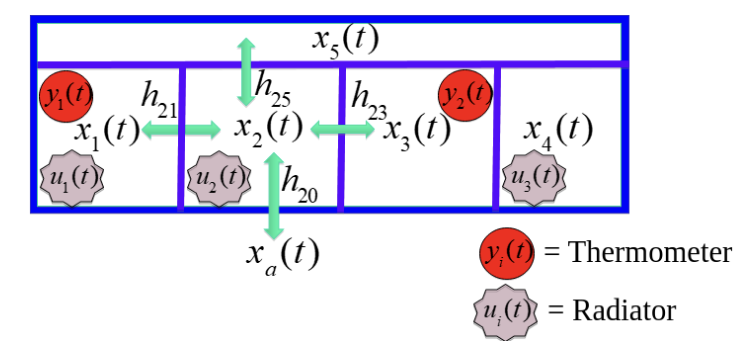
\includegraphics[width=0.5\linewidth]{./figures/building.png}\\
    \textbf{Fig.~2:} Building model schematic
  \end{center}
  \begin{parts}
  \part Write down the dynamical equations of the building in state-space form, including a term for disturbances $d(t)$, and for the ambient temperature $x_a(t)$, assuming the parameters are
    \begin{align}
      \frac{h_{ij}}{C_{i}} &= 
      \begin{cases}
        10  \text{ W/$^\circ$K}& \text{$i$ is adjacent to $j$}\\
        0 & \text{else}
      \end{cases}\\
      C_i &= 1.08\times 10^6 \text{ J/$^\circ$K}
    \end{align}
    \part Consider an LQR cost function of the form
      \begin{align}
        \int_0^{T}\left[(x-\bar{x})^TQ(x-\bar{x}) + u^TRu\right]dt,
      \end{align}
      where $T=24\text{h}\times 60\frac{\text{m}}{\text{h}}\times 60\frac{\text{s}}{\text{m}} = 86400s$ is one day in seconds.
      Set $\bar{x} = 20^\circ$, and write the dynamics in the coordinates
      $z := x-\bar{x}$.
    \part Note that driving the variable $z(t)\to 0$ is therefore equivalent to driving $x(t) \to 20^\circ$.
      Write a \texttt{matlab} script to solve the finite-time horizon LQR problem. Select a positive semi-definite $Q$ and a positive-definite $R$ that gives you ``decent'' results. Assume the initial conditions, disturbance, and ambient temperature follow:
      \begin{align}
        x_i(0) &= 15 - i\times{\text{sign}\{(-1)^i\}}~~~[^\circ\text{ C}]\\
        d(t) &= \max\left[0, 500\sin \left( \dfrac{2\pi t}{86400s} \right)-300\right]~~~[\text{W}]\\
        x_a(t) &= 20^\circ+ 5\sin \left( \dfrac{2\pi t}{86400s} \right)~~~[^\circ\text{ C}]
      \end{align}
      where the sign function is:
      \begin{align}
        \text{sign}(x) = 
        \begin{cases}
          1 & x>0\\
          -1 & x<0\\
          0 & x=0.
        \end{cases}
      \end{align}
    \textbf{Note:} If solving the finite-time problem proves too difficult, feel free to solve the infinite-time problem instead. \texttt{Matlab} has a built-in function called \texttt{lqr} that produces the (constant) gain $K$; read the documentation for details. 
    \part Provide:
      \begin{itemize}
        \item A description of your simulation code
        \item Plots of $d(t)$, $x_a(t)$, $x_i(t)$, and $u(t)$.
        \item A discussion of the effects of varying $Q$ and $R$
      \end{itemize}
  \end{parts}

\end{question}
\begin{solution}
  \begin{parts}
    \part 
    To find the dynamical equations of the building in state-space form,  we have to find the system on the form

    \[
        \dot{x} =Ax+Bu, y = Cx+Du
    \]

    The individual room equations are 

    \[
        C_i \dot{x_i(t)} = \sum_{ j \in \text{neighbors}  }^{ } h_{ij} \left(   x_j(t) - x_i(t) \right) + h_{i0} \left( x_a(t) - x_i(t) \right) + u_i(t) + d_i(t)
    \]
    We rearrange this to get 

    \[
        \dot{x} = \sum_{ j }^{  } \frac{ h_{ij} }{ C_i } \left(   x_j(t) - x_i(t) \right) + \frac{ h_{i0} }{ C_i } \left( x_a(t) - x_i(t) \right) + \frac{ u_i(t) }{ C_i } + \frac{ d_i(t) }{ C_i }
    \]
    
    

    We have 5 rooms, thus 5 states, so 
    $ x(t) = \begin{bmatrix}
            x_1(t)\\
            x_2(t)\\
            x_3(t)\\
            x_4(t)\\
            x_5(t)
        \end{bmatrix}   $
    , 3 controllers that regulate temperature, $ u(t)= \begin{bmatrix}
        u_1(t)\\
        u_2(t)\\
        u_3(t)
    \end{bmatrix}  $ and finally, one disturbance term for every room $d(t) = \begin{bmatrix}
            d_1(t)\\
            d_2(t)\\
            d_3(t)\\
            d_4(t)\\
            d_5(t)
        \end{bmatrix}$
    
    $ \frac{ h_{ij} }{ C_i } = \begin{cases}
      10 W/\degree K\text{, if i adjacent to j}\\
      0\text{, else}
    \end{cases} $ 
    
    This makes. A to be a banded matrix. Since all rooms are adjacent to room 5, the matrix A becomes 

    \[
        A = \begin{bmatrix}
            -  \sum_{ j }^{  } \frac{ h_{1j} }{ C_1 } & \frac{ h_{12} }{ C_1 } &0 &0 &\frac{ h_{15} }{ C_1 } \\
            \frac{ h_{21} }{ C_2 } &  -  \sum_{ j }^{  } \frac{ h_{2j} }{ C_2 } & \frac{ h_{23} }{ C_2 } & 0 & \frac{ h_{25} }{ C_2 } \\
            0 &  \frac{ h_{32} }{ C_3 } &  -  \sum_{ j }^{  } \frac{ h_{3j} }{ C_3 } & \frac{ h_{34} }{ C_3 } & \frac{ h_{35} }{ C_3 } \\
            0 & 0 & \frac{ h_{43} }{ C_4 } &  -  \sum_{ j }^{  } \frac{ h_{4j} }{ C_4 } & \frac{ h_{45} }{ C_4 } \\
            \frac{ h_{51} }{ C_5 } & \frac{ h_{52} }{ C_5 } & \frac{ h_{53} }{ C_5 } & \frac{ h_{54} }{ C_5 } & -  \sum_{ j }^{  } \frac{ h_{5j} }{ C_5 } 
        \end{bmatrix}\\
        = \begin{bmatrix}
            -30 & 10 & 0 &0&10\\
            10&-40&10&0&10\\
            0&10&-40&10&10\\
            0&0&10&-30&10\\
            10&10&10&10&-50
        \end{bmatrix}  
    \]
    Since there are three actuators in rooms 1, 2 and 4, the B matrix is written as 

    \[
        B = \begin{bmatrix}
            \frac{ 1 }{ C_1 }&0&0\\
            0& \frac{ 1 }{ C_2 }&0\\
            0&0&0\\
            0&0& \frac{ 1 }{ C_4 }\\
            0&0&0
        \end{bmatrix}  = \begin{bmatrix}
            \frac{ 1 }{ 1.08\times 10^6 }&0&0\\
            0& \frac{ 1 }{ 1.08\times 10^6 }&0\\
            0&0&0\\
            0&0& \frac{ 1 }{ 1.08\times 10^6 }\\
            0&0&0
        \end{bmatrix} 
    \]
    
    We have the vector b that takes into account the ambient coupling of temperatures. 
    \[
        b = \begin{bmatrix}
           H_{10}\\
           H_{20}\\
           H_{30}\\
           H_{40}\\
           H_{50}\\ 
        \end{bmatrix} = \begin{bmatrix}
           10\\
           10\\
           10\\
           10\\
           10\\ 
        \end{bmatrix}
    \]
    and D is a diagonal matrix with $ \frac{ 1 }{ C_i } = \frac{ 1 }{ 1.08\times 10 ^6 } $ for disturbance inputs.
    
    If we now follow the notes on building control from the lecture slides of optimal control (lecture 4), we obtain the dynamic equations $ \dot{x} = Ax(t)+Bu(t)+bx_a(t)+Dd(t) $ 
    
    

    \part
    
    For this problem, we note that $ z = x-\bar{x} $, then $ x = z + \bar{x} $ and $ \dot{x}= \dot{z} $ since $ \bar{x} $ is a constant temperature of $ 20 \degree C \approx 293 \degree K$ since $ 1\degree C  = 1K$ (K $ = $  Kelvin)     

    so we get the dynamics in thez coordinates as 

    \begin{align*}
      \dot{z} &= A \left( z+ \bar{x} \right) + Bu \\
      &= Az + A\bar{x}+Bu
    \end{align*}
    
    $ A\bar{x} $ can be seen as the forcing term towards the reference temperature in the system.
        
    \part

    Solving the finite-time horizon problem seems to me very hard, as we dont have any initial points to work backwards from. So I just used the infinite-time horizon


    

  \end{parts}
\end{solution}

\begin{question}[10]

Suppose that $Q=\mathbf{0}$, the zero matrix, and $R=I$.
Prove that
\begin{align}
  x_0^TS_0x_0 = \min_{\{u_k\}_{k=0}^{T-1}}\sum_{k=0}^{T-1}\|u_k\|_2^2,
\end{align}
 meaning that $J_0=x_0^TS_0x_0$ is the minimum control energy required to drive the system to zero.
  
\end{question}
\begin{solution}

\end{solution}

 \question[10] \textit{Crassidis \& Junkins} Problem 3.14
\begin{solution}
  
\end{solution}   
 \question[10] \textit{Crassidis \& Junkins} Problem 3.15
\begin{solution}
  
\end{solution}
 \question[10] \textit{Crassidis \& Junkins} Problem 7.4
\begin{solution}
  
\end{solution}

\end{questions}
\end{document}